\section{Implementation and Experiments}
\label{sec:impl&exper}
In this section, we apply our method introduced in Section \ref{sec:attack} to attack the secp256k1 curve in OpenSSL 1.1.1b.
  We implement the Flush+Flush attack  to obtain
the cache side channel information.
The details of the implementation and the result of attacking the elliptic curves are provided.
Then we implement the lattice attacks and solve them by the BKZ lattice reduction algorithm.
 The experiments demonstrate the results of our attacks with different parameters.
Finally, we compare our method with some previous attacks.

%这一章我们展示攻击的具体实现过程,
%对secp256k1进行攻击,曲线的window是3
%实现平台

\subsection{The Flush+Flush Attack}
\label{ffattack}
We test the cache side channel attack on an HP Elite 8300 running Ubuntu 16.04.
The machine features an Intel Core i7-3300 processor with four execution cores and an 8 MB LLC.
The attacking target is the ECDSA implemented in OpenSSL1.1.1b, which uses wNAF representation in the scalar multiplication.
For the experiments, we use the Flush+Flush to attack the 256-bit curve secp256k1.
Followings are the implementation details for the Flush+Flush attack.

%平台

\noindent\textbf{Get the virtual address. }
We use a spy process to monitor the  \verb+EC_POINT_dbl()+,  \verb+EC_POINT_add()+ and \verb+EC_POINT_invert()+ functions in OpenSSL.
So we need to know the virtual addresses of the three functions.
First we get the offsets of the three functions required to monitor in the code of the dynamic library.
Then we use the \verb+mmap()+ function to load each page locating the monitored function codes into the virtual address space of the spy process.
The \verb+mmap()+ function will return the initial address of the page so that we can get the virtual address of the monitored function based on the offset and the address of this page.
Alternative way is to use the \verb+dl_iterate_phdr()+ function to get the initial address of the dynamic library when loaded into the address space.

To determine offsets of the memory lines in the  dynamic library,  we build OpenSSL with debugging symbols.
 These symbols are not loaded at run time and do not affect the performance of the code.
Typically the debugging symbols are not available for attackers,
 however they could use reverse engineering [16] to determine the offsets.



%获取虚拟地址

%首先获取所需监控函数代码在动态库中的偏移量
%接着获取函数代码虚拟地址,有两种方法
%使用mmap()函数,将所监控函数代码所在页加载入地址空间中,获取到函数代码的虚拟地址
%或编译时链接动态库,运行时使用dl_iterate_phdr()函数,获取到动态库加载入地址空间的起始地址,根据偏移量,获得函数代码的虚拟地址
%
%
%
%Victim:通过调用OpenSSL的crypto.so库来进行ECDSA签名运算。
%Attacker:使用和victim相同的crypto库,对victim使用的点加和倍点函数以及EC_POINT_invert()代码所在的cache行进行监控。



\noindent\textbf{Thresholds.}
We monitor the execution time of the \verb+clflush+ instruction to flush the monitored functions.
If the time is larger than the threshold, meaning the memory line is accessed by the victim.
Otherwise, the memory line is not accessed.
The thresholds are calculated for every monitored functions.
For each address of the monitored functions, we record the time of flushing the cache 1000 times, and take the time larger than 99 percent samples plus 6 as the threshold of this address.
The thresholds are recalculated every time before the attack is triggered.


%阈值
%对每个需要监控的地址都计算各自的阈值
%每次监测都重新计算阈值
%对每个地址,监控1000次flush花费的时间,取99%以上样本所花的最大时间加上6作为该地址的阈值


\noindent\textbf{Trigger the monitoring.}
We monitor the execution time of the address of the three functions.
When the time of any one is larger than the corresponding threshold,
 we start to record execution times, meaning that the attack starts.
The record stops when the number of consecutive execution time of all the monitored addresses less than the threshold  is larger than 300.
If the number of record is less than 1000, we re-record the execution time.
Then we have a valid record.
 Due to the  disturbance of noise,
  the valid record does not necessarily contain the activities of the monitored functions in the scalar multiplication.
So we continuously obtain 10 valid records.
%触发
%1) 某一个监控地址的flush时间大于阈值以后,开始记录;
%2)所有地址连续小于阈值的数量大于200后,停止记录;
%3)如果记录数据量小于1000,重新开始记录;
%4)连续记录10次。


\noindent\textbf{Time slot.}
For the attack, the spy process divides time into time slots of approximately $2500$ cycles.
In each slot, the spy flushes the memory lines in the add, double and invert functions (\verb+EC_POINT_dbl()+,  \verb+EC_POINT_add()+ and \verb+EC_POINT_invert()+) out of the caches.
Also, the length of the time slot is chosen to ensure that the three functions only execute once.
This allows the spy to correctly distinguish consecutive doubles.

\noindent\textbf{Determine the initial point.}
In order to precisely recover the sign of the ephemeral key, we need to determine which sample represents the start of the scalar multiplication.
We can determine the
start of the scalar multiplication
by combining the double-and-add chain and the profiles of the double and add functions with wNAF representation.
Also we can determine the start position by monitor the code of copy function in OpenSSL.
 We note that when the computation of scalar multiplication starts, OpenSSL performs the copy function instead of the add function.
 Thus we can monitor the copy function, and when the copy function is called in the time slot and the add function is called in the next slot, it means that the scalar multiplication starts.

%起始判断
%对标量乘法代码分析,在对k的最高位处理时,并不是使用的点加,而是copy,因此,可以对copy函数进行监控,当一个时间槽内进行了倍点和copy操作,可以认定标量乘法的开始。
%如果不监控copy,也可以根据点加倍点的发生,去排除错误的触发;也可以根据NAF编码时点加倍点的特征来判断起始。

\noindent\textbf{Experimental results.}
Fig.~\ref{fig1} shows a fragment of the output of the spy when OpenSSL performs ECDSA with the secp256k1 curve.
In this figure, $\square$, $\lozenge$ and $\vartriangle$ represent ``double", ``add" and ``invert" respectively.
From this fragment, three operations can be clearly distinguished,
 so we success to obtain the ``double-add-invert" chain easily.



%%10次实验
%We totally run 10 experiments, i.e. monitoring the ECDSA signature 10 times.
%The accurate rate is defined as the value of the actual number of bits obtained divided by the ideal number of bits available.
%Thus, from these experiments the average accurate rate of the data obtained from the Flush+Flush attack is xx\%.

\begin{figure}
\centering
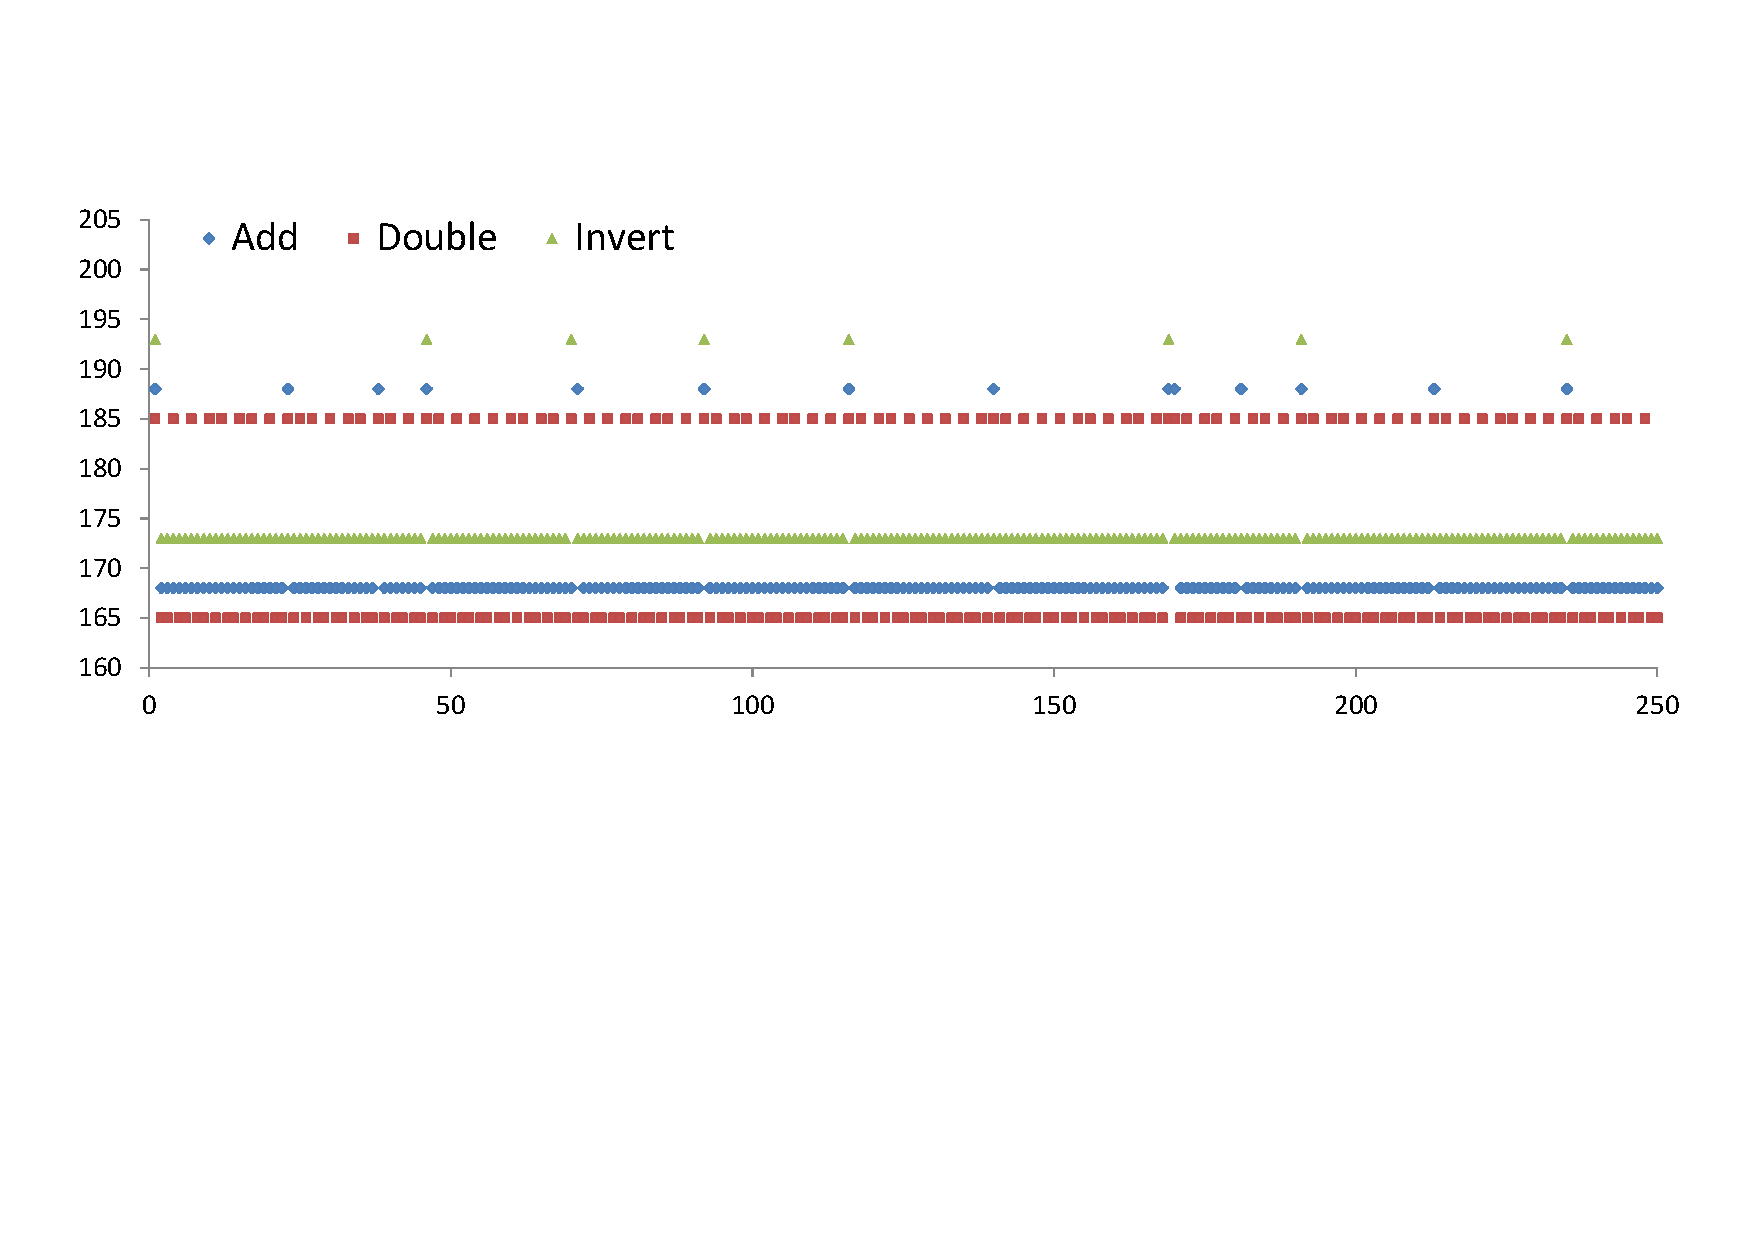
\includegraphics[width=\textwidth]{pic/slot2500.pdf}
\caption{A fragment of the output of the Flush+Flush attack.} \label{fig1}
\end{figure}


%对这个示例进行解释:
%什么符号代表哪个操作
%sample大于阈值xx 表示在这个时间槽内,函数被执行了。
%然后,for example, 对于时间槽1, 什么被访问了,代表哪个函数被执行了,因此对应于0或者1,
%然后时间槽x代表1,
%接着说时间槽x2 代表1,同时invert调用了,说明该位符号和之前相反,
%时间槽x3,未调用invert,符号位和之前相同。
%
%时间槽x4可能是噪声,对噪声的处理
%
%和真实的k相比,正确率是x\%
%
%用ff攻击一条曲线,得到结果,得到double add invert 链,进行恢复
%然后恢复成功率是多少?
%
%
%结果


\subsection{Lattice Attack}
\label{latticeattack}
%使用完美的侧信道结果
%我们的结果是:
%进行分析
%分析为什么我们没有利用全部的信息,理论上怎样,实际怎样
We apply our lattice attack to the curve secp256k1 in our experiments, and we assume that the Flush+Flush attack is perfect, that is we can correctly obtain the ``double-add-invert" chain and recover all the information about the digits of the ephemeral key it contains.

The HNP problem can be solved by exploiting both the CVP and SVP instances.
However, the CVP problem does not have a polynomial time solution while the SVP problem has.
So, with growth of the dimension of the lattice, the time cost of finding the closest vector grows very fast.
 Actually, the CVP problem can be converted to the SVP problem,
  so it is often solved through embedding the CVP into an SVP problem and using the polynomial time solution in practice.
Therefore,
 in our experiments, we only demonstrate the result of using the SVP problem to solve the HNP instance.

 We use the BKZ algorithm implemented in \verb+fplll+~\cite{fplll} to solve the SVP problem.
When solving a SVP instance, there are two outcomes that either we obtain the private key or a wrong answer.
 So we denote the success probability as the amount of successfully recovering the private key divided by the total number of the lattice attacks.
We want to find the optimal strategy for our attack in terms of the following parameters:
\begin{itemize}
%\item CVP or SVP
 \item  lattice dimensions
 \item  the block size of BKZ
 \item  the minimal value of $l$ (length of the consecutive bits of $k$)
 %\item  pruning strategy (optional)
 %\item  total signature number
\end{itemize}

Thus we perform a number of experiments with different values of the parameters.
 In each case we run $200$ experiments and compute the success probability.
Because in Section \ref{sec:attack} the HNP problem introduced requires $l/2 - \log_{2}{3} -1 \geq 1$ to contain more than one bit information, the value of $l$ should be larger than $7$.
 But in our experiments, when $l = 8$, the private key can not be successfully recovered.
  The reason is that the HNP instance contains not enough information.
So the minimal length of the consecutive bits of $k$ is set ranging from $9$ to $11$ in the experiments.
The block size in BKZ is set $10$  and $20$.
The number of sequences of the consecutive bits for constructing the lattice denoted as $d$ is ranged from $50$ to $230$,
i.e. the dimension of the lattice for the SVP is $d + 2$.

\begin{table}[t]
  \centering
  \caption{The success probability of solving SVP with different parameters.}
  \label{svp9}
    \begin{tabular}{|c|c|c|c|}
    \hline
    \multirow{2}{*}{Dimension}&
    \multicolumn{3}{c|}{Block size} \\%&\multicolumn{3}\\ %
    \cline{2-4}
    & 10 & 20 & 30\\
    %\hline
  \hline
  50 & 0 & 0 & 0 \\
  \hline
  60 & 0 & 0 & 1.0 \\
  \hline
  70 & 0.8 & 1.2  & 1.3 \\
  \hline
  80 & 4.3 & 8.6 &  9.7 \\
  \hline
  90 & 14.4 & 22.8 & 23.7 \\
  \hline
  100 & 21.0 & 33.6 & 39.9 \\
  \hline
  110 & 16.3 & 36.7 &  \\
  \hline
  120 & 21.7 & 35.0 &  \\
  \hline
  130 & 24.0 & 45.7 &  \\
  \hline
  140 & 29.0 & 46.3 &  \\
  \hline
  150 & 32.3 & 49.3 &  \\
  \hline
  160 & 27.7 & 49.3 &  \\
  \hline
  170 & 39.0 & 56.7 &  \\
  \hline
  180 & 37.3 & 57.0 &  \\
  \hline
  190 & 39.3 & 63.5 &  \\
  \hline
  200 & 46.0 & 66.0 &  \\
  \hline
  210 & 51.7 & 66.0 &  \\
  \hline
  220 & 51.3 & 72.5 &  \\
  \hline
  230 & 58.7 & 73.5 &  \\
  \hline
    \end{tabular}
\end{table}

Table \ref{svp9} shows the success probability for different dimensions and block sizes of solving the SVP instance in the
             cases that the minimal length of the consecutive bits ranges from $9$ to $11$.
As shown in the table, we successfully retrieve the private key of a 256-bit ECDSA only need $60$ sequences of consecutive bits with the success probability being $1\%$.
These $60$ sequences come from up to $60$ signatures.
Therefore we just need at most $60$ signatures to successfully recover the ECDSA private key.

  For the fixed  minimal length of consecutive bits,
 increasing the dimension generally increases the probability of success.
In some sense, as the dimension increases
     more information is being added to the lattice and this makes the desired solution vector stand out more.
Also, the higher block sizes perform with a higher probability of success,
 as the stronger reduction allows them to isolate the solution vector better.
  We believe that the success probability would be surely higher with the block size $30$ or the BKZ2.0~\cite{bkz2}.

When $l$ is fixed, to get a suitable success probability, attackers can either increase the dimension or use stronger algorithms (increasing the block size).
However, increasing the dimension requires more signatures
 and enlarging the block size increases the computation time.
So attackers can balance the two factors according to their resources and needs.

The success probability also increases as the minimal length of consecutive bits increases.
It is because that more information is added to the lattice making it easier to search for the desired solution vector.
But the increase of the minimal length would lead to require more signatures to obtain enough eligible sequences of consecutive bits,
 because With the increase of minimal length, the probability of obtaining  a longer sequence of consecutive bits becomes lower.


%\begin{table}[b]
%  \centering
%\begin{tabular}{|c|c|c|c|}
%  \hline
%  % after \\: \hline or \cline{col1-col2} \cline{col3-col4} ...
%  dimension & 10 & 20 & 30 \\
%  50 & 0 & 0 & 0 \\
%  60 & 0 & 0 & 1.0 \\
%  70 & 0.8 & 1.2  & 1.3 \\
%  80 & 4.3 & 8.6 &  9.7 \\
%  90 & 14.4 & 22.8 &  \\
%  100 & 21.0 & 33.6 &  \\
%  110 & 16.3 & 36.7 &  \\
%  120 & 21.7 & 35.0 &  \\
%  130 & 24.0 & 45.7 &  \\
%  140 & 29.0 & 46.3 &  \\
%  150 & 32.3 & 49.3 &  \\
%  160 & 27.7 & 49.3 &  \\
%  170 & 39.0 & 56.7 &  \\
%  180 & 37.3 & 57.0 &  \\
%  190 & 39.3 & 63.5 &  \\
%  200 & 46.0 & 66.0 &  \\
%  210 & 51.7 & 66.0 &  \\
%  220 & 51.3 & 72.5 &  \\
%  230 & 58.7 & 73.5 &  \\
%  \hline
%\end{tabular}
%  \caption{the SVP result}\label{svp9}
%\end{table}

%Table \ref{svp8, svp9, svp10} show the probability of success when solving the CVP instance.
%As shown from the table,
%  the number of fragments of consecutive bits that we need to retrieve the private key of a 256-bit ECDSA is only $60$, less than the result of the SVP instance with the low block size.
% The probability of success also increases as the the dimension or the block size increase.
%Moreover, while the minimal length of consecutive bits increases, the probability of success becomes higher.
%%再加一段或几句CVP结果和SVP结果进行比较。


%The results of the SVP and CVP experiments (Appendix A) show that for fixed  minimal length of consecutive bits,
% increasing the dimension generally increases the probability of success.
%In some sense, as the dimension increases more information is being added to the lattice and this makes the desired solution vector stand out more.
%The higher block sizes perform better,
% as the stronger reduction allows them to isolate the solution vector better.
%While the minimal length of consecutive bits increases, the the probability of success become higher.
%Also we see that extensive pre-processing of the basis with more complex lattice reduction techniques provides no real benefit.


\begin{table}[!t]
  \centering
   \caption{Comparison with previous attack methods}\label{compare1}
\begin{tabular}{|c|m{90pt}|c|c|c|}
  \hline
  % after \\: \hline or \cline{col1-col2} \cline{col3-col4} ...
  Methods & The exploited information & HNP or EHNP & \# of bits & \# of signatures \\
  \hline
  Benger et al. \cite{Benger2014} & LSB & HNP & 2 & 200 \\
  \hline
  van de Pol et al. \cite{Van2015} & half positions of non-zero digits & HNP & 47.6 & 13 \\
  \hline
  Fan et al. \cite{Fan2016} & all positions of non-zero digits & EHNP & 105.8 & 4 \\
  \hline
  Wang et al. \cite{Wang2017} & positions of two non-zero digits and the length of the wNAF representation of $k$ & HNP & $\geq$ 2.99 & 85 \\
  \hline
  Ours & all positions and signs of non-zero digits & HNP & 154.2  & $\leq$ 60 \\
%  \hline
%  190 & 39.3 & 63.5 & & \\
  \hline
\end{tabular}
\end{table}

\subsection{Comparison with Other Attack Methods}
\label{compare}

 Generally,  to attack the ECDSA implementation with the wNAF representation,
   the attackers target the implementation of scalar multiplication
      and use cache side channel attacks to achieve the information about the ephemeral key $k$.
Through side channels attackers can get a ``double-and-add" chain for the scalar multiplication.
However,
 it is hard to directly recover the whole ephemeral key just depending on the ``double-and-add" chain.
From the obtained information it can recover partial bits of the ephemeral key.
Hence attackers exploit the incomplete information of $k$ to transform the problem of private key recovery into one that can be solved by lattice, such as HNP or EHNP problem.
 Then the attackers retrieve the private key by solving the HNP or EHNP problem through being converted to the CVP/SVP problem in the lattice.

We compare the previous attack methods with ours in several aspects and the result is shown in Table \ref{compare1}.

Benger et al. \cite{Benger2014} got the least significant bits (LSBs) of the ephemeral key through the Flush+Reload attack
although this is not all the information obtained from the side channel.
Then they used the LSBs of many signatures to construct a HNP problem and
successfully retrieved the private key by solving the CVP/SVP instance of a specific lattice converted from the HNP problem.
The number of bits extracted from each signature is very small, only an average of 2 bits information can be obtained.
Thus made it require more than $200$ signatures to recover a 256-bit private key with the probability being $3.5\%$.
In our work, we exploit information from the cache side channel to extract the consecutive bits at the position of every non-zero bits for the ephemeral key.
All the consecutive bits can be used to construct the lattice attack.
Therefore, we can get much more bits per signature and the number of signatures is decreased for retrieve the private key.

van de Pol et al. \cite{Van2015} improved Benger's attack  relying on the property of some specific elliptic curves, that is the order $q$ of the base point is a pseudo-Mersenne prime which can be expressed as $2^n - \epsilon$, where $|\epsilon| < 2^p $, $p \approx n/2$.
With this property, this attack uses the information from the consecutive non-zero digits whose positions are between $p+1$ and $n$ extracted from the Flush+Reload attack, not only the LSBs.
It is able to extract $47.6$ bits per signature on average for the secp256k1 curve and recover the private key with 13 signatures.
Then they constructed a new HNP instance using this information and
successfully retrieved the private key.
Although this work greatly reduced the number of signatures needed to recover the private key,
the information from the cache side channel is not fully utilized.
But our work can use all the information from the cache side channel.
Moreover, their work is only effective to some special curves,
 but ours can be applied to all the curves without any restriction.
%This means that they can use about half of the information they got from the side channel.


Fan et al.\cite{Fan2016} extract all positions of digits from the Flush+Reload attack and take advantage of them to construct an EHNP instance.
They managed to obtain on average 105.8 bits per signature for the secp256k1 curve
 and only need 4 signatures to retrieve the private key with the probability being $8\%$.
 Compared with their work, ours obtains more information about the ephemeral key, i.e. the sign of all non-zero digits, from the side channel by analysing the OpenSSL implementation.
We can extract 154.2 bits information per signature.
Although it uses more signatures to retrieve the private key through our lattice attack,
theoretically the number of signatures needed is less than Fan's if a suitable lattice is constructed.

Wang et al. \cite{Wang2017} obtain the positions of two non-zero digits and the length of the wNAF representation of $k$ from the Flush+Reload attack.
They can obtain no less than 2.99 bits information per signature and exploit the HNP to recover the private key for the 256-bit curve using $85$ signatures.
Obviously, our method obtains more information and uses less signatures to recover the private key.

In summary, our method obtain the sign and the position of the ephemeral key $k$ from the Flush+Flush attack.
It can extract the largest amount of data, on average $154.2$ bits information per signature.
In theory, the number of signatures need to retrieve the private key is $2$.
  However, due to the limit of our method of lattice construction, we need at most $60$ signatures, which is more than Fan's and van's.


%2017年,范团队还在science China information sciences 上发了一篇,使用HNP的文章,
%这是一个b类的期刊。(交叉综合新兴)
%我们比这个期刊的文章效果要好的。




























